\section{Implementation of a Proof of Concept}




\subsection{Description of the proof of concept}

Our proof of concept aims at demonstrating of how quantum annealing can be considered as an alternative to classical methods in the solution of food production optimization. Since, as explained previously, advantage has not been proven or disproved, we will limit ourselves and report results and findings.


\subsection{Benchmarking Strategies}

Our benchmark consists of two main components: \textbf{scenarios} and \textbf{solvers}.

We will test two solvers, namely the state of the art open source python library for Linear Programs, PuLP (which can run solvers like Gurobi \cite{gurobi2023} and CPLEX \cite{cplex2023}) and the D-Wave Leap Hybrid Solver, to maintain a direct comparison in case we detect any possibility of \textit{local advantage}.

We don't know how the Hybrid Solver operates in detail, but to try to understand better where quantum computing might help us, we can consider how our problem can be decomposed:

\paragraph{Benders Decomposition:}

We solve the mixed-integer problem by partitioning the binary selection variables $\mathbf{Y}$ (the master) from the continuous allocation variables $\mathbf{A}$ (the subproblem). The original compact problem is:

\begin{align}
\min_{A,Y}\quad & -Z(A) + \mathbf{d}^T Y
    && \text{(equivalently maximize $Z$)} \\
\text{s.t.}\quad
& \sum_{c} A_{f,c} \le L_f
    && \forall f \\
& A_{f,c} \ge A^{\min}_c\, Y_{f,c}, \quad
  A_{f,c} \le L_f\, Y_{f,c}
    && \forall f,c \\
& FG^{\min}_g \le \sum_{f}\sum_{c\in G_g} Y_{f,c} \le FG^{\max}_g
    && \forall g \\
& A_{f,c} \ge 0,\quad Y_{f,c}\in\{0,1\}.
\end{align}


For a fixed candidate $\bar Y$ the subproblem is an LP in $\mathbf{A}$:

\begin{align}
\phi(\bar Y) = \min_{A \ge 0}\; & -Z(A) \\
\text{s.t.}\quad
& \sum_{c} A_{f,c} \le L_f && \forall f, \\
& A_{f,c} \ge A^{\min}_c\,\bar Y_{f,c}, \quad
  A_{f,c} \le L_f\,\bar Y_{f,c} && \forall f,c.
\end{align}


Dual information from the subproblem produces feasibility cuts when the subproblem is infeasible and optimality cuts when it is feasible; these cuts are added to the master, which can be written compactly as:

\begin{equation}
\begin{aligned}
\min_{Y \in {0,1}^{\cdot},;\theta} \quad
& \mathbf{d}^T Y + \theta \\
\text{s.t.}\quad
& \text{(food-group and other combinatorial constraints on $Y$)} \\
& \theta \ge \beta^k + \sum_{f,c} \alpha^k_{f,c} Y_{f,c}
\quad \text{for each optimality cut }k, \\
& \text{feasibility cuts (when generated).}
\end{aligned}
\end{equation}

The practical iterative procedure is given in Algorithm \ref{alg:benders} below.
\begin{algorithm}[H]
\caption{Benders Decomposition Algorithm}
\label{alg:benders}
\begin{algorithmic}[1]
\State \textbf{Initialize:} Master problem with no cuts; iteration counter $k \gets 0$.
\Repeat
\State Solve the master MILP to obtain candidate binary vector $\bar{Y}^{(k)}$ and master estimate $\theta^{(k)}$.
\State Solve the subproblem LP for fixed $\bar{Y}^{(k)}$:
\If{subproblem is \textbf{infeasible}}
\State Obtain an infeasibility ray and derive a feasibility cut.
\State Add the cut to the master and go to Step 2.
\Else
\State Subproblem is feasible; compute $\phi(\bar{Y}^{(k)})$ and extract corresponding dual variables.
\State Construct an optimality cut using the duals and add it to the master.
\EndIf
\State Evaluate the optimality gap: $|\theta^{(k)} - \phi(\bar{Y}^{(k)})|$.
\If{gap $\le$ tolerance}
\State \textbf{Stop:} Current solution is optimal.
\Else
\State $k \gets k + 1$.
\EndIf
\Until{convergence}
\end{algorithmic}
\end{algorithm}



\begin{table}[ht]
\centering
\caption{Notation and symbols}
\label{tab:notation}
\small
\begin{tabular}{@{} l p{8.5cm} l @{}} \toprule
\textbf{Symbol} & \textbf{Meaning} & \textbf{Domain / notes} \\ \midrule
$A_{f,c}$ & Area (continuous) allocated on farm $f$ to crop $c$. & $A_{f,c}\ge0$ (continuous) \\
$Y_{f,c}$ & Binary selection: 1 if crop $c$ is planted on farm $f$, 0 otherwise. & $Y_{f,c}\in\{0,1\}$ \\
$\mathbf{A},\:\mathbf{Y}$ & Stacked vectors/matrices of $A_{f,c}$ and $Y_{f,c}$ respectively. & — \\
$Z(A)$ & Continuous part of the objective (e.g., profit or yield) as a function of $A$. & sign convention: you minimize $-Z(A)$ in the model \\ 
$\mathbf{d}$ & Vector of coefficients multiplying $Y$ in the objective (fixed costs or penalties). & $\mathbf{d}^T\mathbf{Y}$ appears in master objective \\ 
$L_f$ & Total land (available area) on farm $f$. & scalar, farm-local upper bound \\ 
$A^{\min}_c$ & Minimum area required for crop $c$ if selected on a farm. & used in coupling: $A_{f,c}\ge A^{\min}_c Y_{f,c}$ \\ 
$G_g$ & Set of crops that belong to food-group $g$. & index set \\ 
$FG^{\min}_g,\; FG^{\max}_g$ & Lower and upper bounds on the number of plantings (or coverage) for food-group $g$. & Integers or counts over $f,c\in G_g$ \\ 
$\bar Y$ (or $\bar Y^{(k)}$) & Candidate binary vector returned by the master at an iteration (trial solution). & fixed when solving subproblem \\ 
$\phi(\bar Y)$ & Optimal value of the subproblem (LP) for fixed $\bar Y$. & finite if subproblem feasible; otherwise indicates infeasibility \\ 
$\theta$ & Auxiliary master variable that lower-bounds the subproblem value ($\theta\ge\phi(\cdot)$ via cuts). & continuous scalar in master \\ 
$\alpha^k_{f,c}$ & Coefficients of $Y_{f,c}$ in optimality cut $k$ (derived from dual solution). & appear in $\theta \ge \beta^k + \sum_{f,c}\alpha^k_{f,c}Y_{f,c}$ \\ 
$\beta^k$ & Constant (intercept) term in optimality cut $k$ (from duals and constants). & constant offset in cut $k$ \\ 
$\pi_f$ & Dual multiplier for farm-level land constraint $\sum_c A_{f,c}\le L_f$. & $\pi_f\ge0$ (depending on convention) \\ 
$f$ & Index for farms (element of index set $\mathcal{F}$). & discrete index \\
$c$ & Index for crops (element of index set $\mathcal{C}$). & discrete index \\
$g$ & Index for food-groups (element of index set $\mathcal{G}$). & discrete index \\
$k$ & Index for Benders cuts / iterations (cut counter). & integer iteration / cut index \\
infeasibility ray & Dual ray produced when the subproblem is infeasible; used to form feasibility cuts. & yields linear inequality in $Y$ \\ \bottomrule
\end{tabular}
\end{table}

From preliminary benchmarking of the classical and hybrid solvers across multiple scenarios and strategies, (Farms vs Patches, Non-linear Numerator vs Denominator), we can see from Figure \ref{fig:comprehensive_quality_analysis} what the relative advantages are. These results show that while there is a spectrum of performances in terms of speed across the models, with the classical PuLP formulations being best, there is potential advantage to be obtained in the quality of the solution from the hybrid solver especially with the patch approach where we have a more complex and realistic ``plot assignment" model where each discrete patch of land can only be assigned to a single crop. The nearly constant QPU usage time also suggests that for growing problem sizes or complexity, there is a speed advantage to be found for the hybrid solvers due to the worse scaling of the classical solvers.

\begin{figure}[t]
    \centering
    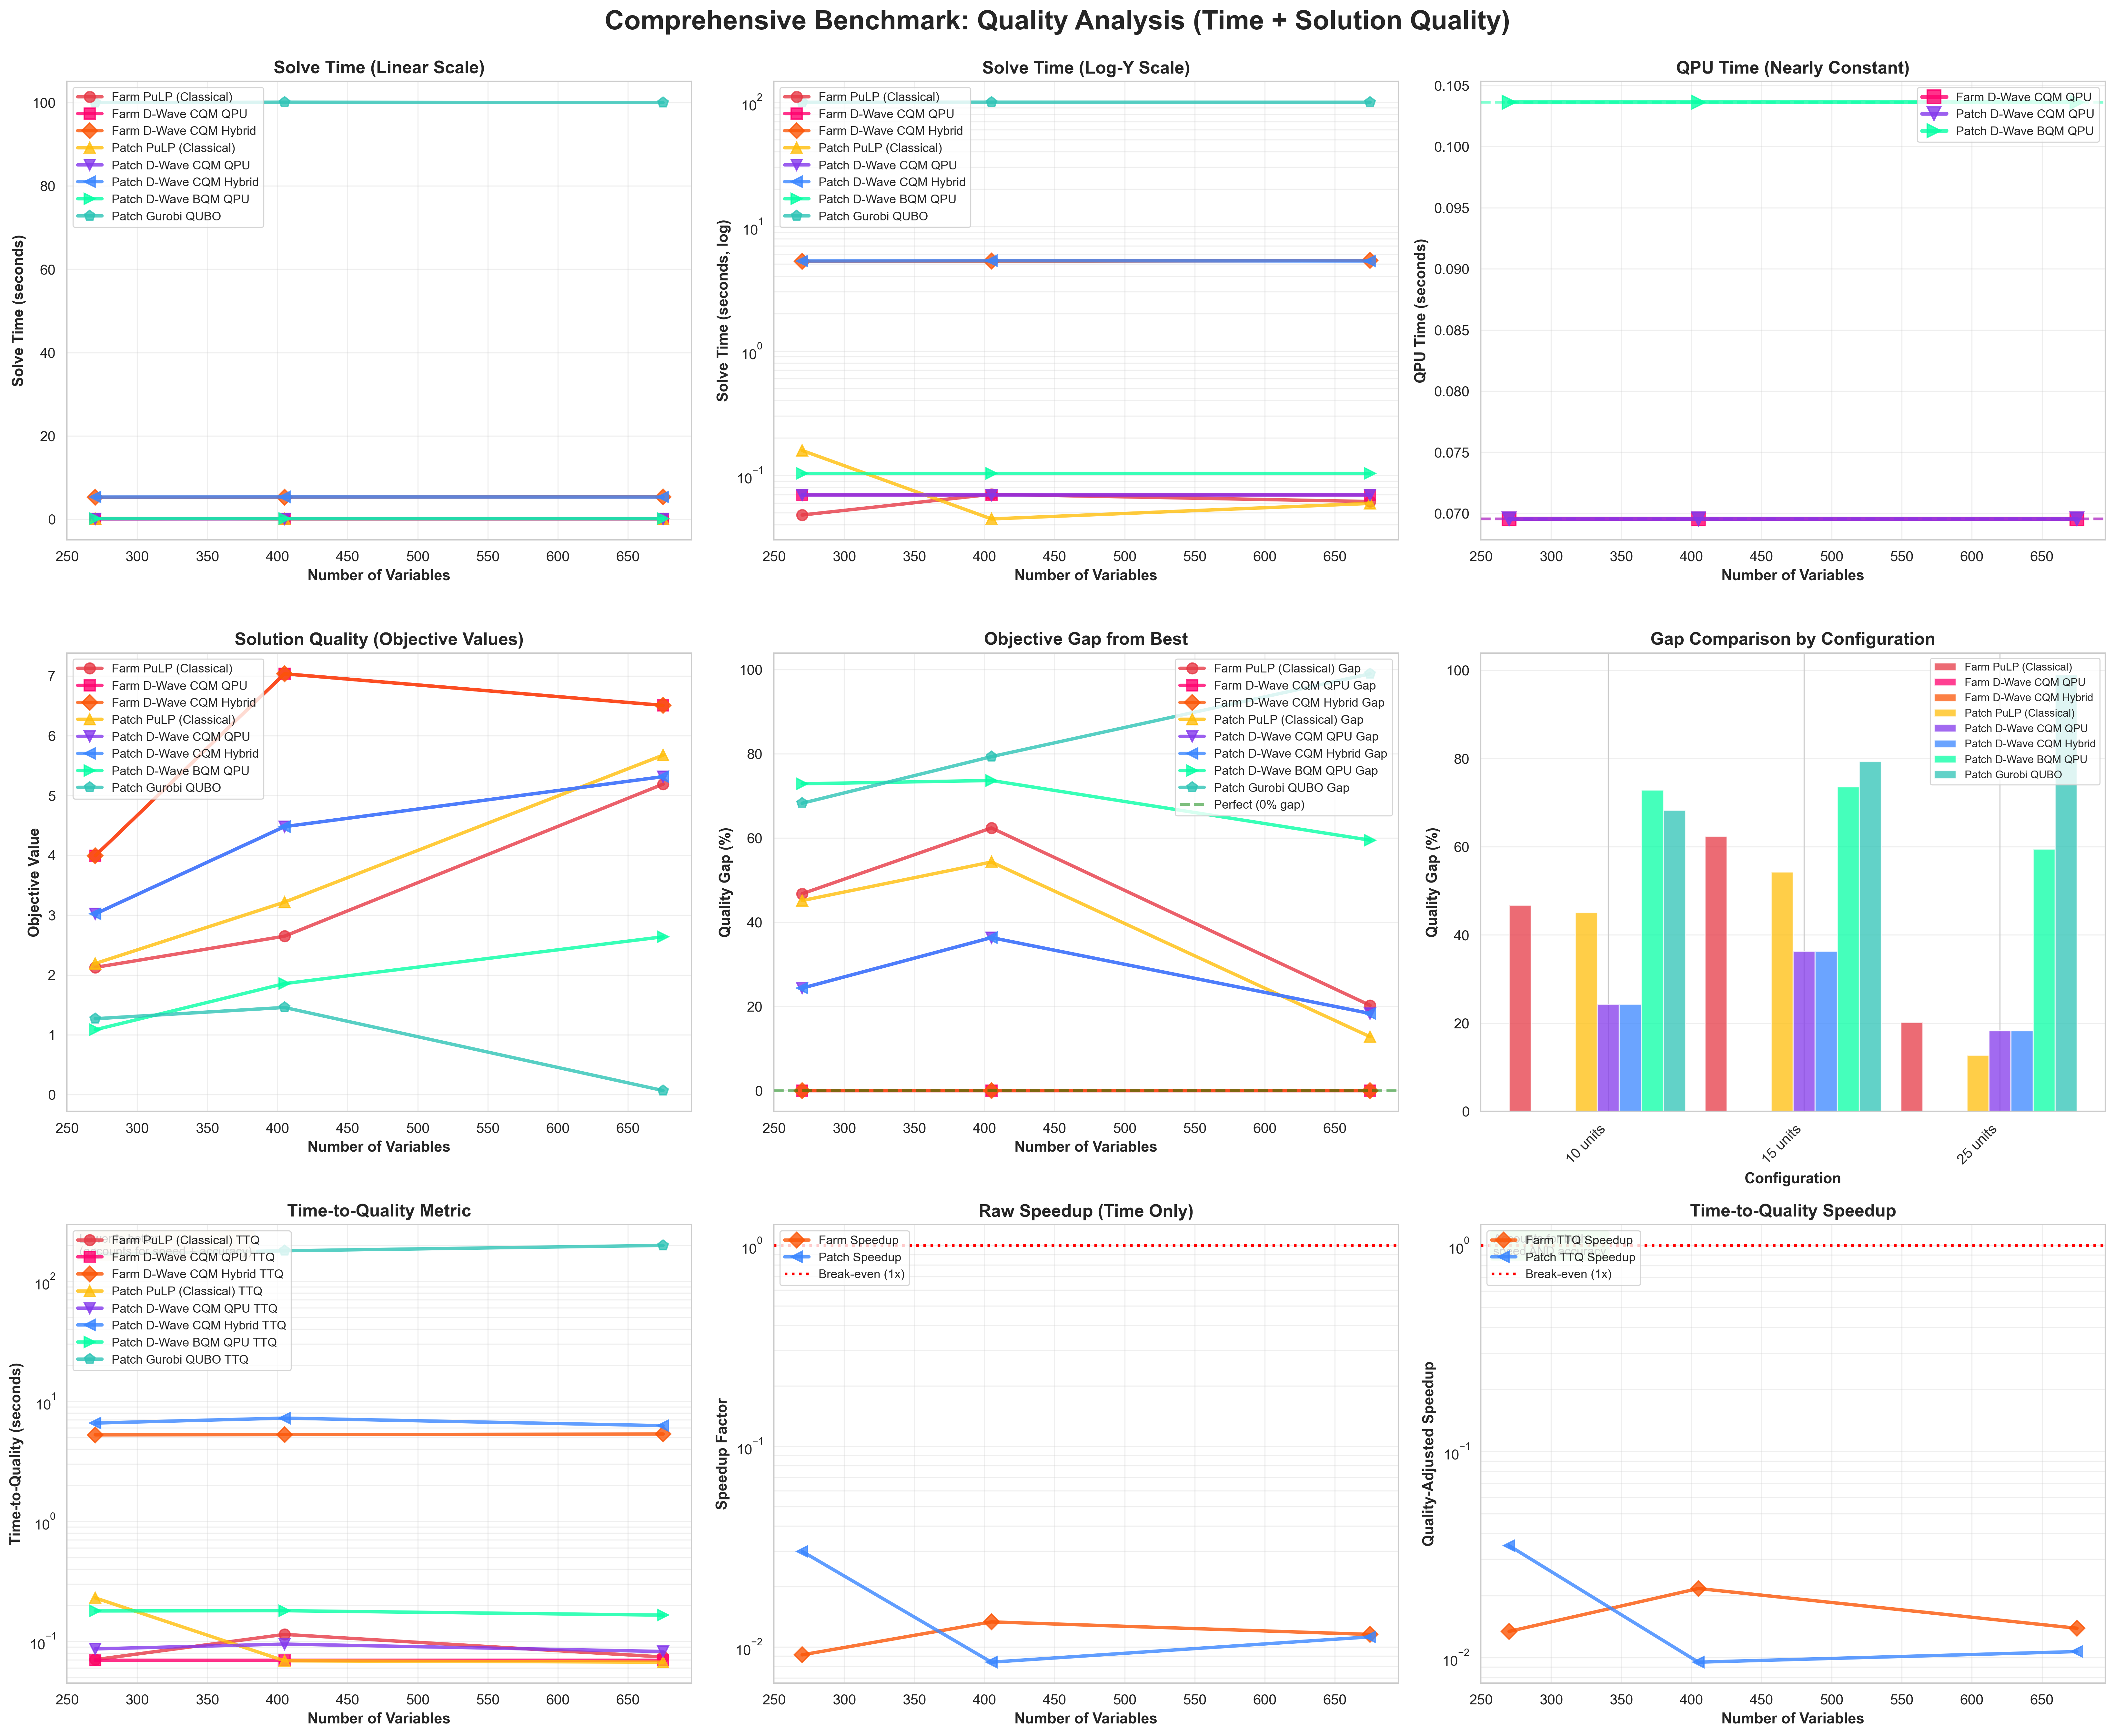
\includegraphics[width=\textwidth]{Figures/comprehensive_quality_analysis.png}
    \caption{Preliminary Benchmark Results for Classical and Hyrbid Solvers.}
    \label{fig:comprehensive_quality_analysis}
\end{figure}


\subsection{Resource Estimation}


\textbf{Overview:}  
 Problems scale from 18 to 500+ variables, with hybrid solvers best suited for constrained formulations.

\medskip
\textbf{Problem Sizes Tested:}

\begin{center}
\begin{tabular}{@{}lllll@{}}
\toprule
Level & Vars & Farms & Foods & Density \\
\midrule
Simple        & 10  & 2 & 5  & 0.333 \\
Intermediate  & 18  & 3 & 6  & 0.333 \\
Full          & 50  & 5 & 10 & 0.200 \\
\bottomrule
\end{tabular}
\end{center}

\medskip
\textbf{Scaling:}
\begin{itemize}
    \item Linear fit: $T \approx 0.0059V - 0.04$
    \item Exponential: $T \approx 0.006e^{0.076V}$
    \item Scope: 50 vars (current) $\to$ 100--200 (extended) $\to$ 500+ (scalability)
\end{itemize}

\medskip
\textbf{Resource Estimates:}

\begin{center}
\begin{tabular}{@{}llll@{}}
\toprule
Size & QPU Time & Embedding & Hybrid Time \\
\midrule
Small ($\leq$20)  & 2--100 ms  & 1--5 s   & 10--60 s \\
Medium (20--100)  & 10--200 ms & 5--30 s  & 30--180 s \\
Large (100+)      & 20--500 ms & 30--120 s & 60--600+ s \\
\bottomrule
\end{tabular}
\end{center}

\medskip
\textbf{Upper Bounds (95th \%ile):}

\begin{center}
\begin{tabular}{@{}llll@{}}
\toprule
Size & QPU (s) & Hybrid (s) & Wall Time (s) \\
\midrule
$\leq$50   & $\leq$0.5 & $\leq$300  & $\leq$360 \\
50--200    & $\leq$2   & $\leq$900  & $\leq$1080 \\
200--500   & $\leq$5   & $\leq$3600 & $\leq$4320 \\
\bottomrule
\end{tabular}
\end{center}

\medskip
\textbf{Architecture:}
\begin{itemize}
    \item \emph{Hybrid (CQM)}: continuous + binary vars, LeapHybridCQMSampler
    \item \emph{Pure QPU}: QUBO, EmbeddingComposite + D-WaveSampler
    \item \emph{Decomposition}: master (hybrid) + farm subproblems (QPU)
\end{itemize}

\medskip
\textbf{Risks \& Mitigations:}
\begin{itemize}
    \item Embedding limits $\to$ hybrid/decomposition
    \item Local minima $\to$ multiple runs
    \item Runtime inflation $\to$ simplify/limit time
\end{itemize}

\medskip
\textbf{Recommendations:}
\begin{itemize}
    \item Start: 18-variable tests (5--15 min/exp.)
    \item 1-hour allocation: 6--12 small, 2--4 medium, 1--2 large
    \item Safety margins: $\times$2 time, $\times$1.5 samples, +50\% buffer
\end{itemize}

\medskip
\textbf{Conclusion:}  
Hybrid solvers provide robustness (5--40 min/exp). QPU scaling predictable; 1-hour budget supports baseline validation, comparisons, and scalability demos.



\subsection{Steps to Achieve a Proof of Concept}


\subsubsection{}{Key Data Inputs and Requirements}



\begin{enumerate}


\item{Population and Nutritional Needs}
\begin{itemize}
    \item \textbf{Demographics:} Age, gender, height, weight, pregnant and lactating women (PLW)
    \item \textbf{Population projections:} Projected population growth and demographic breakdown
    \item \textbf{Nutritional requirements:} Calories, protein, dietary fats, essential micronutrients for each population group:
    \begin{itemize}
        \item Infants
        \item Boys and girls
        \item Adolescent boys and girls
        \item Men and women of reproducing age
        \item Pregnant and lactating women
        \item Elderly
    \end{itemize}
\end{itemize}

\item{Food System Requirements}
\begin{itemize}
    \item \textbf{Culturally acceptable foods:} Foods produced and consumed within the local food system context (Diet Quality Questionnaire Database)
    \item \textbf{Food basket design:} Identification of food combinations that fulfill all nutritional needs
    \item \textbf{GAIN nLCA score:} To optimize for nutrition and environment (GHGs, water, land use)
    \item \textbf{Cost analysis:} Cheapest sources of good nutrition per nutritional unit using Nutritional Value Score
\end{itemize}


\item{Production Feasibility Analysis}
\begin{itemize}
    \item \textbf{Crop production requirements:}


\begin{itemize}
    \item Total quantity of each crop required
    \item Yield per hectare of selected/local/optimal varieties
    \item Total land available for crop production
    \item Preferred production methods and compatibility with local climate, soil, and water availability
    \item Compatibility of different crops within the same cultivated area
\end{itemize}

\item \textbf{Animal-source food production:}
\begin{itemize}
    \item Total quantity required for meat, dairy, eggs, poultry, seafood
    \item Total production potential and yield from fisheries
    \item Compatibility of production methods with local systems
    \item Integration potential with crop systems
\end{itemize}
\end{itemize}

\end{enumerate}


\subsubsection{Scenario Creation}

\paragraph{Crops:}

The data were provided by GAIN in three different datasets:
\begin{itemize}
    \item \path{LCA results per kg & NVS.xlsx}
    \item \path{NVS_12Apr2024.xlsx}
    \item \path{PricePer100NVS_Indonesia_3Sept2024.xlsx}
\end{itemize}


The values were processed as follows to obtain normalized values:  

\begin{itemize}
    \item 
    \begin{equation}
       \text{Env. Impact}=\left(\frac{\text{NVS}}{100}\times\frac{\text{Primary\_production\_mPt\_100NVS}}{\max(\text{Primary\_production\_mPt\_100NVS})}\right)
    \end{equation}
    \item 
    \begin{equation}
       \text{Sustainability}=\left(\frac{\text{NVS}}{100}\times\frac{\text{TOTAL\_categories\_mPt\_100NVS}}{\max(\text{TOTAL\_categories\_mPt\_100NVS})}\right)^{-1}
    \end{equation}
    \item
    \begin{equation}
       \text{Affordability}=\left(\frac{\text{NVS}}{100}\times\frac{\text{Cost to achieve NVS score of 100}}{\max(\text{Cost to achieve NVS score of 100})}\right)^{-1}
    \end{equation}
\end{itemize}

To create a comprehensive dataset, the same food was found in all three files (manually due to different naming conventions). Then all rows containing empty values were discarded and the columns aggregated.

The data for the complete scenario is represented below:
\begin{table}[ht]
\centering
\scriptsize
\label{tab:food_data}
\begin{tabular}{llrrrrr}
\toprule
\textbf{Food\_Name} & \textbf{Food Group}      & \textbf{Nut. Val.} & \textbf{Nut. Den.} & \textbf{Sust.} & \textbf{Env. Imp.} & \textbf{Afford.} \\
\midrule
Mango          & Fruits                & 0.4468 & 0.2458 & 0.0757 & 0.0044 & 0.0261 \\
Papaya         & Fruits                & 0.4754 & 0.2748 & 0.1778 & 0.0172 & 0.0398 \\
Orange         & Fruits                & 0.4707 & 0.2537 & 0.1280 & 0.0083 & 0.0254 \\
Banana         & Fruits                & 0.4195 & 0.1963 & 0.1140 & 0.0088 & 0.0801 \\
Guava          & Fruits                & 0.5156 & 0.3102 & 0.1791 & 0.0120 & 0.0570 \\
Watermelon     & Fruits                & 0.3111 & 0.0706 & 0.0833 & 0.0089 & 0.0152 \\
Apple          & Fruits                & 0.3710 & 0.0884 & 0.0776 & 0.0045 & 0.0133 \\
Avocado        & Fruits                & 0.4674 & 0.2455 & 0.0511 & 0.0026 & 0.0357 \\
Durian         & Fruits                & 0.4516 & 0.2483 & 0.0275 & 0.0016 & 0.0203 \\
Corn           & Starchy staples       & 0.3908 & 0.1535 & 0.1214 & 0.0113 & 0.4179 \\
Potato         & Starchy staples       & 0.4782 & 0.3053 & 0.1246 & 0.0113 & 0.0934 \\
Tofu           & Pulses, nuts, and seeds & 0.5211 & 0.3471 & 0.1052 & 0.0188 & 0.1026 \\
Tempeh         & Pulses, nuts, and seeds & 0.5391 & 0.3946 & 0.1115 & 0.0201 & 0.2248 \\
Peanuts        & Pulses, nuts, and seeds & 0.4650 & 0.4268 & 0.0546 & 0.0031 & 0.2678 \\
Chickpeas      & Pulses, nuts, and seeds & 0.5153 & 0.3286 & 0.1404 & 0.0125 & 0.3980 \\
Pumpkin        & Vegetables            & 0.5889 & 0.4766 & 0.0579 & 0.0030 & 0.0338 \\
Spinach        & Vegetables            & 0.9032 & 0.9346 & 0.0859 & 0.0043 & 0.0362 \\
Tomatoes       & Vegetables            & 0.5816 & 0.4394 & 0.1039 & 0.0061 & 0.0387 \\
Long bean      & Vegetables            & 0.5616 & 0.4127 & 0.0821 & 0.0047 & 0.3634 \\
Cabbage        & Vegetables            & 0.6376 & 0.5007 & 0.0791 & 0.0043 & 0.0341 \\
Eggplant       & Vegetables            & 0.3967 & 0.1731 & 0.0597 & 0.0035 & 0.0217 \\
Cucumber       & Vegetables            & 0.4306 & 0.2272 & 0.1058 & 0.0084 & 0.0188 \\
Egg            & Animal-source foods   & 0.5837 & 0.4851 & 0.0343 & 0.0017 & 0.0217 \\
Beef           & Animal-source foods   & 0.5968 & 0.5424 & 0.0038 & 0.4468 & 0.0241 \\
Lamb           & Animal-source foods   & 0.5941 & 0.5332 & 0.0088 & 0.0005 & 0.0242 \\
Pork           & Animal-source foods   & 0.5840 & 0.5233 & 0.0165 & 0.0008 & 0.3743 \\
Chicken        & Animal-source foods   & 0.5533 & 0.4336 & 0.0249 & 0.0013 & 0.0572 \\
\bottomrule
\end{tabular}
\caption{Food Data Overview}
\end{table}

\newpage
\paragraph{Farms:}

The farms were added to each scenario by sampling this distribution, obtained from \cite{LOWDER201616}.

\begin{table}[h!]
\centering

\begin{tabular}{lcc}
\toprule
\textbf{Size class (ha)} & \textbf{Share of farms (\%)} & \textbf{Share of land (\%)} \\
\midrule
$<1$        & $\sim 45$ & $\sim 10$ \\
$1$--$2$    & $\sim 20$ & $\sim 10$ \\
$2$--$5$    & $\sim 15$ & $\sim 20$ \\
$5$--$10$   & $\sim 8$  & $\sim 15$ \\
$10$--$20$  & $\sim 5$  & $\sim 20$ \\
$>20$       & $\sim 7$  & $\sim 25$ \\
\bottomrule
\end{tabular}
\caption{Distribution of farm sizes and land shares in the Global South}
\label{tab:farm_size_distribution}
\end{table}


\paragraph{Weights:}

Weights combinations are used to follow an \textit{a posteriori} decision policy: multiple weights configurations are tested per scenario and based on the objective value obtained, the preferred configuration is chosen by the centralized decisionmakers
